
%% bare_conf.tex
%% V1.3
%% 2007/01/11
%% by Michael Shell
%% See:
%% http://www.michaelshell.org/
%% for current contact information.
%%
%% This is a skeleton file demonstrating the use of IEEEtran.cls
%% (requires IEEEtran.cls version 1.7 or later) with an IEEE conference paper.
%%
%% Support sites:\documentclass[10pt]{•}
%% http://www.michaelshell.org/tex/ieeetran/
%% http://www.ctan.org/tex-archive/macros/latex/contrib/IEEEtran/
%% and
%% http://www.ieee.org/

%%*************************************************************************
%% Legal Notice:
%% This code is offered as-is without any warranty either expressed or
%% implied; without even the implied warranty of MERCHANTABILITY or
%% FITNESS FOR A PARTICULAR PURPOSE! 
%% User assumes all risk.
%% In no event shall IEEE or any contributor to this code be liable for
%% any damages or losses, including, but not limited to, incidental,
%% consequential, or any other damages, resulting from the use or misuse
%% of any information contained here.
%%
%% All comments are the opinions of their respective authors and are not
%% necessarily endorsed by the IEEE.
%%
%% This work is distributed under the LaTeX Project Public License (LPPL)
%% ( http://www.latex-project.org/ ) version 1.3, and may be freely used,
%% distributed and modified. A copy of the LPPL, version 1.3, is included
%% in the base LaTeX documentation of all distributions of LaTeX released
%% 2003/12/01 or later.
%% Retain all contribution notices and credits.
%% ** Modified files should be clearly indicated as such, including  **
%% ** renaming them and changing author support contact information. **
%%
%% File list of work: IEEEtran.cls, IEEEtran_HOWTO.pdf, bare_adv.tex,
%%                    bare_conf.tex, bare_jrnl.tex, bare_jrnl_compsoc.tex
%%*************************************************************************

% *** Authors should verify (and, if needed, correct) their LaTeX system  ***
% *** with the testflow diagnostic prior to trusting their LaTeX platform ***
% *** with production work. IEEE's font choices can trigger bugs that do  ***
% *** not appear when using other class files.                            ***
% The testflow support page is at:
% http://www.michaelshell.org/tex/testflow/



% Note that the a4paper option is mainly intended so that authors in
% countries using A4 can easily print to A4 and see how their papers will
% look in print - the typesetting of the document will not typically be
% affected with changes in paper size (but the bottom and side margins will).
% Use the testflow package mentioned above to verify correct handling of
% both paper sizes by the user's LaTeX system.
%
% Also note that the "draftcls" or "draftclsnofoot", not "draft", option
% should be used if it is desired that the figures are to be displayed in
% draft mode.
%
\documentclass[conference]{IEEEtran}
\usepackage{german}
\usepackage[utf8]{inputenc}
\usepackage[T1]{fontenc}
\usepackage{dblfloatfix}
\usepackage{amsmath}
\usepackage{amssymb}
\usepackage{threeparttable}
\usepackage{graphicx}
\usepackage[justification=centering, margin=0.5cm]{caption}
\usepackage{subfig}
% Add the compsoc option for Computer Society conferences.
%
% If IEEEtran.cls has not been installed into the LaTeX system files,
% manually specify the path to it like:
% \documentclass[conference]{../sty/IEEEtran}





% Some very useful LaTeX packages include:
% (uncomment the ones you want to load)


% *** MISC UTILITY PACKAGES ***
%
%\usepackage{ifpdf}
% Heiko Oberdiek's ifpdf.sty is very useful if you need conditional
% compilation based on whether the output is pdf or dvi.
% usage:
% \ifpdf
%   % pdf code
% \else
%   % dvi code
% \fi
% The latest version of ifpdf.sty can be obtained from:
% http://www.ctan.org/tex-archive/macros/latex/contrib/oberdiek/
% Also, note that IEEEtran.cls V1.7 and later provides a builtin
% \ifCLASSINFOpdf conditional that works the same way.
% When switching from latex to pdflatex and vice-versa, the compiler may
% have to be run twice to clear warning/error messages.






% *** CITATION PACKAGES ***
%
%\usepackage{cite}
% cite.sty was written by Donald Arseneau
% V1.6 and later of IEEEtran pre-defines the format of the cite.sty package
% \cite{} output to follow that of IEEE. Loading the cite package will
% result in citation numbers being automatically sorted and properly
% "compressed/ranged". e.g., [1], [9], [2], [7], [5], [6] without using
% cite.sty will become [1], [2], [5]--[7], [9] using cite.sty. cite.sty's
% \cite will automatically add leading space, if needed. Use cite.sty's
% noadjust option (cite.sty V3.8 and later) if you want to turn this off.
% cite.sty is already installed on most LaTeX systems. Be sure and use
% version 4.0 (2003-05-27) and later if using hyperref.sty. cite.sty does
% not currently provide for hyperlinked citations.
% The latest version can be obtained at:
% http://www.ctan.org/tex-archive/macros/latex/contrib/cite/
% The documentation is contained in the cite.sty file itself.






% *** GRAPHICS RELATED PACKAGES ***
%
\ifCLASSINFOpdf
  % \usepackage[pdftex]{graphicx}
  % declare the path(s) where your graphic files are
  % \graphicspath{{../pdf/}{../jpeg/}}
  % and their extensions so you won't have to specify these with
  % every instance of \includegraphics
  % \DeclareGraphicsExtensions{.pdf,.jpeg,.png}
\else
  % or other class option (dvipsone, dvipdf, if not using dvips). graphicx
  % will default to the driver specified in the system graphics.cfg if no
  % driver is specified.
  % \usepackage[dvips]{graphicx}
  % declare the path(s) where your graphic files are
  % \graphicspath{{../eps/}}
  % and their extensions so you won't have to specify these with
  % every instance of \includegraphics
  % \DeclareGraphicsExtensions{.eps}
\fi
% graphicx was written by David Carlisle and Sebastian Rahtz. It is
% required if you want graphics, photos, etc. graphicx.sty is already
% installed on most LaTeX systems. The latest version and documentation can
% be obtained at: 
% http://www.ctan.org/tex-archive/macros/latex/required/graphics/
% Another good source of documentation is "Using Imported Graphics in
% LaTeX2e" by Keith Reckdahl which can be found as epslatex.ps or
% epslatex.pdf at: http://www.ctan.org/tex-archive/info/
%
% latex, and pdflatex in dvi mode, support graphics in encapsulated
% postscript (.eps) format. pdflatex in pdf mode supports graphics
% in .pdf, .jpeg, .png and .mps (metapost) formats. Users should ensure
% that all non-photo figures use a vector format (.eps, .pdf, .mps) and
% not a bitmapped formats (.jpeg, .png). IEEE frowns on bitmapped formats
% which can result in "jaggedy"/blurry rendering of lines and letters as
% well as large increases in file sizes.
%
% You can find documentation about the pdfTeX application at:
% http://www.tug.org/applications/pdftex





% *** MATH PACKAGES ***
%
%\usepackage[cmex10]{amsmath}
% A popular package from the American Mathematical Society that provides
% many useful and powerful commands for dealing with mathematics. If using
% it, be sure to load this package with the cmex10 option to ensure that
% only type 1 fonts will utilized at all point sizes. Without this option,
% it is possible that some math symbols, particularly those within
% footnotes, will be rendered in bitmap form which will result in a
% document that can not be IEEE Xplore compliant!
%
% Also, note that the amsmath package sets \interdisplaylinepenalty to 10000
% thus preventing page breaks from occurring within multiline equations. Use:
%\interdisplaylinepenalty=2500
% after loading amsmath to restore such page breaks as IEEEtran.cls normally
% does. amsmath.sty is already installed on most LaTeX systems. The latest
% version and documentation can be obtained at:
% http://www.ctan.org/tex-archive/macros/latex/required/amslatex/math/





% *** SPECIALIZED LIST PACKAGES ***
%
%\usepackage{algorithmic}
% algorithmic.sty was written by Peter Williams and Rogerio Brito.
% This package provides an algorithmic environment fo describing algorithms.
% You can use the algorithmic environment in-text or within a figure
% environment to provide for a floating algorithm. Do NOT use the algorithm
% floating environment provided by algorithm.sty (by the same authors) or
% algorithm2e.sty (by Christophe Fiorio) as IEEE does not use dedicated
% algorithm float types and packages that provide these will not provide
% correct IEEE style captions. The latest version and documentation of
% algorithmic.sty can be obtained at:
% http://www.ctan.org/tex-archive/macros/latex/contrib/algorithms/
% There is also a support site at:
% http://algorithms.berlios.de/index.html
% Also of interest may be the (relatively newer and more customizable)
% algorithmicx.sty package by Szasz Janos:
% http://www.ctan.org/tex-archive/macros/latex/contrib/algorithmicx/




% *** ALIGNMENT PACKAGES ***
%
%\usepackage{array}
% Frank Mittelbach's and David Carlisle's array.sty patches and improves
% the standard LaTeX2e array and tabular environments to provide better
% appearance and additional user controls. As the default LaTeX2e table
% generation code is lacking to the point of almost being broken with
% respect to the quality of the end results, all users are strongly
% advised to use an enhanced (at the very least that provided by array.sty)
% set of table tools. array.sty is already installed on most systems. The
% latest version and documentation can be obtained at:
% http://www.ctan.org/tex-archive/macros/latex/required/tools/


%\usepackage{mdwmath}
%\usepackage{mdwtab}
% Also highly recommended is Mark Wooding's extremely powerful MDW tools,
% especially mdwmath.sty and mdwtab.sty which are used to format equations
% and tables, respectively. The MDWtools set is already installed on most
% LaTeX systems. The lastest version and documentation is available at:
% http://www.ctan.org/tex-archive/macros/latex/contrib/mdwtools/


% IEEEtran contains the IEEEeqnarray family of commands that can be used to
% generate multiline equations as well as matrices, tables, etc., of high
% quality.


%\usepackage{eqparbox}
% Also of notable interest is Scott Pakin's eqparbox package for creating
% (automatically sized) equal width boxes - aka "natural width parboxes".
% Available at:
% http://www.ctan.org/tex-archive/macros/latex/contrib/eqparbox/





% *** SUBFIGURE PACKAGES ***
%\usepackage[tight,footnotesize]{subfigure}
% subfigure.sty was written by Steven Douglas Cochran. This package makes it
% easy to put subfigures in your figures. e.g., "Figure 1a and 1b". For IEEE
% work, it is a good idea to load it with the tight package option to reduce
% the amount of white space around the subfigures. subfigure.sty is already
% installed on most LaTeX systems. The latest version and documentation can
% be obtained at:
% http://www.ctan.org/tex-archive/obsolete/macros/latex/contrib/subfigure/
% subfigure.sty has been superceeded by subfig.sty.



%\usepackage[caption=false]{caption}
%\usepackage[font=footnotesize]{subfig}
% subfig.sty, also written by Steven Douglas Cochran, is the modern
% replacement for subfigure.sty. However, subfig.sty requires and
% automatically loads Axel Sommerfeldt's caption.sty which will override
% IEEEtran.cls handling of captions and this will result in nonIEEE style
% figure/table captions. To prevent this problem, be sure and preload
% caption.sty with its "caption=false" package option. This is will preserve
% IEEEtran.cls handing of captions. Version 1.3 (2005/06/28) and later 
% (recommended due to many improvements over 1.2) of subfig.sty supports
% the caption=false option directly:
%\usepackage[caption=false,font=footnotesize]{subfig}
%
% The latest version and documentation can be obtained at:
% http://www.ctan.org/tex-archive/macros/latex/contrib/subfig/
% The latest version and documentation of caption.sty can be obtained at:
% http://www.ctan.org/tex-archive/macros/latex/contrib/caption/




% *** FLOAT PACKAGES ***
%
%\usepackage{fixltx2e}
% fixltx2e, the successor to the earlier fix2col.sty, was written by
% Frank Mittelbach and David Carlisle. This package corrects a few problems
% in the LaTeX2e kernel, the most notable of which is that in current
% LaTeX2e releases, the ordering of single and double column floats is not
% guaranteed to be preserved. Thus, an unpatched LaTeX2e can allow a
% single column figure to be placed prior to an earlier double column
% figure. The latest version and documentation can be found at:
% http://www.ctan.org/tex-archive/macros/latex/base/



%\usepackage{stfloats}
% stfloats.sty was written by Sigitas Tolusis. This package gives LaTeX2e
% the ability to do double column floats at the bottom of the page as well
% as the top. (e.g., "\begin{figure*}[!b]" is not normally possible in
% LaTeX2e). It also provides a command:
%\fnbelowfloat
% to enable the placement of footnotes below bottom floats (the standard
% LaTeX2e kernel puts them above bottom floats). This is an invasive package
% which rewrites many portions of the LaTeX2e float routines. It may not work
% with other packages that modify the LaTeX2e float routines. The latest
% version and documentation can be obtained at:
% http://www.ctan.org/tex-archive/macros/latex/contrib/sttools/
% Documentation is contained in the stfloats.sty comments as well as in the
% presfull.pdf file. Do not use the stfloats baselinefloat ability as IEEE
% does not allow \baselineskip to stretch. Authors submitting work to the
% IEEE should note that IEEE rarely uses double column equations and
% that authors should try to avoid such use. Do not be tempted to use the
% cuted.sty or midfloat.sty packages (also by Sigitas Tolusis) as IEEE does
% not format its papers in such ways.





% *** PDF, URL AND HYPERLINK PACKAGES ***
%
%\usepackage{url}
% url.sty was written by Donald Arseneau. It provides better support for
% handling and breaking URLs. url.sty is already installed on most LaTeX
% systems. The latest version can be obtained at:
% http://www.ctan.org/tex-archive/macros/latex/contrib/misc/
% Read the url.sty source comments for usage information. Basically,
% \url{my_url_here}.





% *** Do not adjust lengths that control margins, column widths, etc. ***
% *** Do not use packages that alter fonts (such as pslatex).         ***
% There should be no need to do such things with IEEEtran.cls V1.6 and later.
% (Unless specifically asked to do so by the journal or conference you plan
% to submit to, of course. )


% correct bad hyphenation here
\hyphenation{op-tical net-works semi-conduc-tor}


\begin{document}
%
% paper title
% can use linebreaks \\ within to get better formatting as desired
\title{Spatial Trajectory Privacy: Comparison of Anonymization Approaches}


% author names and affiliations
% use a multiple column layout for up to three different
% affiliations
%\author{	
%	\IEEEauthorblockN{Alexander Baumgärtner}
% %	\IEEEauthorblockA{Otto-Friedrich Universität\\
%		Bamberg\\
%		Telefon: 0176/30767807}
	
%	\and
		
%	\IEEEauthorblockN{Tina Kämmerer}
%	\IEEEauthorblockA{
%		Otto-Friedrich Universität\\
%		Bamberg, Deutschland}
%	}

 \author{
 	\IEEEauthorblockN{Alexander Baumgärtner, Tina Kämmerer, Lars Taubmann}
 	\IEEEauthorblockA{
 			Mobile Software Systems Seminar\\
 			Otto-Friedrich Universität Bamberg\\
 			Bamberg, Deutschland\\
 			Email: (alexander-wilhelm.baumgaertner, tina-maria.kaemmerer, lars-thomas.taubmann)@stud.uni-bamberg.de}
 }
% conference papers do not typically use \thanks and this command
% is locked out in conference mode. If really needed, such as for
% the acknowledgment of grants, issue a \IEEEoverridecommandlockouts
% after \documentclass

% for over three affiliations, or if they all won't fit within the width
% of the page, use this alternative format:
% 
%\author{\IEEEauthorblockN{Michael Shell\IEEEauthorrefmark{1},
%Homer Simpson\IEEEauthorrefmark{2},
%James Kirk\IEEEauthorrefmark{3}, 
%Montgomery Scott\IEEEauthorrefmark{3} and
%Eldon Tyrell\IEEEauthorrefmark{4}}
%\IEEEauthorblockA{\IEEEauthorrefmark{1}School of Electrical and Computer Engineering\\
%Georgia Institute of Technology,
%Atlanta, Georgia 30332--0250\\ Email: see http://www.michaelshell.org/contact.html}
%\IEEEauthorblockA{\IEEEauthorrefmark{2}Twentieth Century Fox, Springfield, USA\\
%Email: homer@thesimpsons.com}
%\IEEEauthorblockA{\IEEEauthorrefmark{3}Starfleet Academy, San Francisco, California 96678-2391\\
%Telephone: (800) 555--1212, Fax: (888) 555--1212}
%\IEEEauthorblockA{\IEEEauthorrefmark{4}Tyrell Inc., 123 Replicant Street, Los Angeles, California 90210--4321}}




% use for special paper notices
%\IEEEspecialpapernotice{(Invited Paper)}




% make the title area

% IEEEtran.cls defaults to using nonbold math in the Abstract.
% This preserves the distinction between vectors and scalars. However,
% if the conference you are submitting to favors bold math in the abstract,
% then you can use LaTeX's standard command \boldmath at the very start
% of the abstract to achieve this. Many IEEE journals/conferences frown on
% math in the abstract anyway.

% no keywords




% For peer review papers, you can put extra information on the cover
% page as needed:
% \ifCLASSOPTIONpeerreview
% \begin{center} \bfseries EDICS Category: 3-BBND \end{center}
% \fi
%
% For peerreview papers, this IEEEtran command inserts a page break and
% creates the second title. It will be ignored for other modes.
\maketitle


\begin{abstract}
	%\boldmath
	Privatsphäre und Datenschutz stellen wichtige Herausforderungen bei der Verwendung von Location-based Services da. Durch Data Mining und die Verknüpfung mit zusätzlichen Daten können viele private Informationen über einen User gewonnen werden. Um dies zu vermeiden und die Privatsphäre zu schützen existieren eine Vielzahl verschiedener Anonymisierungsansätze, welche Position oder Spatial Trajectory eines Users verschleiern. Diese Arbeit wird drei dieser Ansätze detaillierter darstellen. Zu Beginn werden die Methoden Spatial Cloaking, Mix Zones und False Locations vorgestellt. Im zweiten Abschnitt werden die betrachteten Ansätze gegenüber gestellt und anhand verschiedener Kriterien miteinander verglichen. 
\end{abstract}
\IEEEpeerreviewmaketitle

Keywords—trajectory; location privacy; anonymization; spatial cloaking; dummy trajectory; location-based services
\section{Introduction} \label{sec:introduction}
Ziel dieses Papers ist es, verschiedene Ansätze für die Anonymisierung von Spatial Trajectories vorzustellen und zu vergleichen. Hierzu folgt zunächst ein Überblick über die Thematik Location-based Services (LBS) und die damit einhergehende Problematik des Datenschutzes, anschließend daran werden ergänzende und weiterführende Arbeiten vorgestellt. Im Hauptteil des Papers werden verschiedene Methoden für die Anonymisierung von Spatial Trajectories erläutert und anhand mehrerer Aspekte miteinander verglichen. Zum Abschluss (Kurzes Stichwort für die Conclusion)

Die Kategorie der Location-based Services umfasst eine Vielzahl an mobilen Diensten, die auf Basis der Position des Nutzers selektierte Informationen und Dienste bereit stellen. Vor allem bedingt durch die zunehmende Verbreitung von Smartphones und der damit verbundenen Möglichkeit, auf Standortdaten der Nutzer zuzugreifen, ist die LBS-Branche in Deutschland in den letzten Jahren enorm gewachsen, wie eine Studie der Bayerischen Landeszentrale für neue Medien zeigt \cite{Consulting2014}. Demnach stieg alleine die Zahl der LBS-Anbieter im Zeitraum von 2012 bis 2014 von 130 auf 927 Anbieter. Dabei werden LBS vor allem in den Bereichen Tourismus (z.B. Yelp) und Verkehr (z.B. Öffi) genutzt, aber auch im sozialen Bereich (z.B. Foursquare, Google Latitude), im Einkauf (z.B. Kaufda, Barcoo) und im Gebiet der pervasive Games (z.B. Ingress, Geocaching, Killer).

Allen Anwendungsgebieten zu eigen ist jedoch die Problematik des Datenschutzes, welche durch die Erfordernis und Verwendung von Nutzerdaten. Dies ist besonders kritisch bei kontinuierlichen LBS, welche regelmäßige Updates der Nutzerposition erfordern, da hierbei Benutzerdaten durch räumliche und zeitliche Korrelation der Trajectories erschlossen werden können \cite{Chow2011}. Dieser Aspekt ist auch für die Nutzer relevant: Laut Studie verwenden zwar 67\% der Nutzer LBS, aber nur 36\% davon fühlen sich dabei sicher.



\section{Related Work} \label{sec:realatedWork}
RelatedWork
\section{Approach} \label{sec:approach}
Im Folgenden werden drei verschiedene Methoden für die Anonymisierung von Spatial Trajectories vorgestellt: Spatial Cloaking, Space Tranformation und False Locations.
\subsection{Spatial Cloaking (Alexander Baumgärtner)} \label{sec:spatialCloaking}
Spatial Cloaking ist eine Verschleierungstaktik, bei der der Anwender seinen genauen Standort mithilfe von k-anonymity [1] verheimlicht. Das bedeutet, dass versucht wird eine definierte Fläche zu erzeugen. Diese Fläche soll die Eigenschaft besitzen, dass mindestens k-1 andere Personen sich in dieser aufhalten können. Um dem Anwender eine einfache Möglichkeit zu bieten, seinen Standort zu verschleiern, wird ein sog. locatin anonymizer zwischen den Nutzer und den Locationbased Service (LBS) geschaltet. \\ Stellt der Nutzer nun eine Anfrage an einen Service wie z. B. \"Zeige mir alle Restaurants in der Nähe\", dann schickt das Endgerät seinen genauen Standort mit Anfrage an den Positionsanonymisierer. Dieser erzeugt nun ein Areal, in welchem der Nutzer sich befindet und welches gleichzeitig die Sicherheitskriterien erfüllt. Anschließend stellt der location anonymizer die Anfrage an den vom Nutzer spezifizierten Service, jedoch wird lediglich das Areal und nicht die genaue Position des Anwenders übermittelt. Als Antwort erhält der Positionsanonymisierer nun alle Restaurants in dem Gebiet und kann dem Nutzer alle daraus relevanten Informationen zur Verfügung stellen.\\ Wird im Folgenden von einem Gebiet oder Areal gesprochen, welches von einem Positonsanonyisierer erzeugt wurde, wird[so spricht man von einem Cloaked...] dieses Cloaked-Area genannt. Um eine Cloaked-Area zu erzeugen gibt es verschiedene Methoden. Zum einen [wo ist das zum anderen?] kann der Anonymisierer, wenn er eine sog. Cloaked-Area erzeugen möchte, bei jeder Anfrage an das LBS dieselben Partner verwenden oder [hier zum anderen?] er hat die Möglichkeit sich jedes Mal neue Partner für die Erzeugung einer Cloaked-Area zu suchen. Jedoch ist es bei beiden Methoden nicht ausreichend, zu einem bestimmten Abfragezeitpunkt an den angefragten Service k-anonymität zu gewährleisten [Zitat]. Im Folgenden werden zwei verschiedene Angriffe (trajectory tracing attack und anonymity-set tracing attack) auf das Spatial Cloaking Verfahren erläutert und wie der Nutzer sich gegen diese verteidigen kann. 
\subsubsection{Trajectory tracing Attacke} 
Die trajectory tracing Attacke kann verwendet werden, sollte der Anonymisierer immer dieselben Partner zur Erzeugung einer Cloaked-Area verwenden.[Es ist sinnvoll die trajectory tracting Attacke zu verwenden, wenn der Anonymisierer immer dieselben Partner zur Erzeugung einer Cloaked-Area verwendet] Dabei versucht der Angreifer das Opfer anhand seiner Anfragen an das LBS zu identifizieren, indem ein Schnittpunkt zwischen dem aktuellen Gebiet und dem Gebiet, in welchem er sich seit der letzten Anfrage befinden muss, errechnet wird. Angenommen es wird zum Zeitpunkt t1 eine Cloaked-Area a1 mit den Usern A, B und C erstellt und die Bewegungsgeschwindigkeit von Opfer A ist dem Angreifer bekannt. So kann der Angreifer zu jedem beliebigen nachfolgendem Zeitpunkt tn das maximale Gebiet errechnen, in welchem sich der Nutzer aufhalten kann. Dies muss unter der Berücksichtigung von Straßen- und Geländeverhältnissen geschehen. Daraus ergibt sich zum Zeitpunkt tn eine maximale Grenze. Zu einem Zeitpunkt t2 formt die Gruppe eine neue Spatial-Cloaking-Area a2 und stellt erneut Anfragen an das LBS. Der Angreifer hat nun die Möglichkeit die maximale Grenze vom Zeitpunkt t1 mit a2 zu schneiden. Sollte nur ein Nutzer in dieser Schnittmenge enthalten sein, so hat der Angreifer User A erfolgreich identifiziert.\\  Der Anonymisierer hat zwei Möglichkeiten sich gegen diese Art von Angriff zu wehren. Bei beiden Gegenmaßnahmen muss der Nutzer die maximale Grenze in Abhängigkeit des Zeitpunkt t1 berechnen. Anschließend kann er entweder die \textbf{patching technique} oder die\textbf{delaying technique} anwenden. 
\begin{itemize} 
\item{delaying technique} funktioniert, indem der Anwender eine Anfrage zu einem beliebigen Zeitpunkt t2 an die LBS formuliert. Würde der Anonymisierer nun direkt die Anfrage abschicken, dann könnte der Angreifer die trajectory tracing Attacke durchführen und so den User identifizieren. [Um dies zu verhindern?]Deswegen muss die Anfrage verzögert werden. Die Zeit der Verzögerung ist so groß[Die Verzögerung muss so groß gewählt werden, damit die maximale Grenze von t1 so stark angewachsen ist, bis...], bis die maximale Grenze, bezogen auf t1, so stark angewachsen ist bis diese die gebildete Cloaked-Area a2 zum Zeitpunkt t2 komplett überlappt. Wird nun die Schnittmenge aus a2 und der maximalen Grenze zu t1 errechnet,[so stellt diese das Ergebnis der maximalen Grenze zu t1 dar] ist das Ergebnis die maximale Grenze zu t1. Problematisch sind bei diesem Lösungsansatz jedoch, dass Anfragen an das LBS nicht zeitnah beantwortet werden können. Es gibt immer eine gewisse Wartezeit. \item{patching technique} kombiniert die maximale Grenze basierend auf t1 mit der Cloaked-Area a2, um eine neue Cloaked-Area zu erhalten, welche als Grundlage bei der Anfrage des LBS benutzt wird. Bei dieser Methode leidet jedoch die Genauigkeit der Ergebnisse, da diese neue Cloaked-Area sehr groß werden kann, wenn sich die Personen der Cloaked Area voneinander weg bewegen.  
\end{itemize} 
\subsubsection{anonymity-set tracing Attacke} 
Die zweite Möglichkeit wie ein Angreifer sein Opfer identifizieren kann, ist mithilfe der anonymity-set tracing Attacke. Hierzu muss das Opfer bei jeder Anfrage an das LBS die Cloaked-Area mit anderen Partnern neu erzeugen. Hat der Angreifer nun zwei Anfragen an das LBS mitgelesen, so kann er vergleichen, welche Personen in der Cloaked-Area gleich geblieben sind und welche neu hinzugekommen, bzw. den Bereich verlassen haben. Tritt der Fall ein, dass nur noch eine einzelne Person über alle Cloaked-Areas konstant bleibt, so ist diese Person das Opfer[der Sicherheitsattacke?].\\ Um diesem Angriff entgegen zu wirken, können drei verschiedene Verschleierungstaktiken verwendet werden. Dabei ist es nicht relevant, ob es sich bei den dazu verendeten Daten um Real-Time-Daten handelt, also ob sich zum Zeitpunkt der Erstellung einer Cloaked-Area weitere Personen in der Nähe befinden oder nicht oder[ob es sich um] historische Daten handelt. Außerdem muss ein sog. location anonymizer zwischen dem LBS und dem Anwender platziert werden. Dieser stellt die eigentliche Anfrage an das LBS, um eine Anonymität des Nutzers zu gewährleisten. 
\subsubsection{Group-based Ansatz} 
Der group-based Ansatz ist eine Verschleierungstaktik, welcher[welche?] auf Real-Time Daten aufbaut. Stellt dieselbe Person eine zwei [eine oder zwei?]verschiedene Abfragen an den location anonymizer, so wird die Cloaked-Area immer mit denselben Personen erzeugt, welche auch schon bei der ersten Cloaked-Area involviert waren. So wird sichergestellt, dass die anonymity-set tracing Attacke für einen potentiellen Angreifer nicht anwendbar ist.\\Wenn diese Art von Ansatz gewählt wird um seine Position zu verschlüsseln, so muss man jedoch Nachteile berücksichtigen. Der location anonymizer muss so die Position von allen Nutzern zu jedem Zeitpunkt kennen. Das kann vor allem bei mobilen Endgeräten Probleme mit der Akkulaufzeit verursachen.  
\subsubsection{Distortion-based Ansatz} 
Der distortion-based Ansatz ist eine Erweiterung des group-based Ansatzes. Er versucht das Problem des ständigen online seins aus dem group-based Ansatz zu beheben. Hierzu versucht der Anonymisierer die Position von Nutzern vorher zu sagen. Dazu benutzt dieser die letzte bekannte Position und Geschwindigkeit der einzelnen Personen. Nun muss nur der Nutzer, welcher wirklich eine Anfrage stellt, seinen Standort dem Anonymisierer verraten und es kann dadurch trotzdem eine k-anonymität gewährleistet werden. [Umgangssprache, satz besser formulieren] 
\subsubsection{Predication-based Ansatz} 
Dieser Ansatz benötigt keine Echtzeitinformationen von anderen Nutzern. Ein für ein bestimmtes Gebiet zuständiger Anonymisierer speichert sich dazu die Standorte von verschiedenen Nutzern, welche sich zu einer beliebigen Zeit eingeloggt haben. Soll der location anonymizer nun für einen Nutzer k-anonymität gewährleisten, hat aber nicht genug Personen in dem entsprechendem Gebiet, so greift dieser auf zuvor gespeicherte trajectorys zurück. Problematisch ist jedoch die optimale Fläche der Cloaked-Area zu berechnen, da ein Suchalgorithmus implementiert werden muss, welcher die besten Positionen von aufgezeichneten trajectorys ermittelt. Hier sollte mit einer guten Heuristic gearbeitet werden. 

\subsection{Mix-Zones (Lars Taubmann)} \label{sec:mixZones}
Das Bedrohungsmodel des theoretisch idealen Mix-Zone Konzeptes \cite{Beresford2003} geht davon aus, dass der Benutzer eines LBS diesem nicht traut. Um aber diesen Service dennoch in Anspruch zu nehmen,  bedient er sich eines Middleware Systems, welches als Proxy zwischen dem Nutzer und dem LBS dient. Das Middleware System unterstützt ihn dabei, seine Identität zu verstecken, indem der Nutzer nur Service Callbacks über das Middleware System und in bestimmten dafür definierten Bereichen empfängt. Dafür meldet der Nutzer Interesse an für ihn relevante LBS bei der Middleware an und diese prüft periodisch den Ort des Nutzers und bestimmt, ob für den Nutzer ein relevantes Event ausgelöst worden ist und reicht ihm die Callbacks zu angemessenen Zeitpunkten weiter. Der Middleware Proxy benutzt Pseudonyme um die Identität des Nutzers vor dem Service zu verstecken.

Da Langzeitpseudonyme es ermöglichen, die Identität des Nutzer über spezifisches Verhalten, wie das Aufhalten an bestimmten Orten wie Zuhause oder auf Arbeit, zu ermitteln, schlägt \cite{Beresford2003} einen ständigen Pseudonymwechsel vor, auch wenn der Nutzer getrackt wird. Die Middleware versorgt den Nutzer regelmäßig mit neuen, unbenutzten Pseudonymen für jede ortssensible Anwendung. Dieser Pseudonymwechsel findet innerhalb der sogenannten Mix-Zone statt. Allerdings können nur LBS genutzt werden, die Pseudonyme unterstützen.

Das Konzept der Mix-Zone wird aus dem Konzept der Mix-Nodes aus dem Bereich der anonymen Kommunikationssystemen abgeleitet \cite{Chow2011}. Die Idee, die hinter dem Mix-Node liegt ist, dass er wartet bis er k Pakete mit gleicher Länge empfangen hat und diese, bevor er sie weiter leitet, zufällig oder nach einer Metrik neu sortiert, so dass eine Unverknüpfbarkeit zwischen eingehenden und ausgehenden Paketen  entsteht.

\cite{Beresford2003} definiert eine Mix-Zone für eine Nutzergruppe als eine zusammenhängende Region mit maximaler Größe, in der keiner dieser Benutzer den Callback eines LBS erhalten hat. Für diese Nutzergruppe können mehrere unterschiedliche Mix-Zones bestehen. Das Gegenstück zu einer Mix-Zone ist die Application Zone, als Gebiet, in der ein Nutzer einen Callback empfangen hat. Der Middleware Proxy kann die Mix-Zones im Voraus oder für jede Nutzergruppe einzeln als Gebiet festlegen, in dem sich gerade kein Stück einer Application Zone befindet.

Weil standortbasierte Anwendungen in Mix-Zones keine ortsbezogenen Informationen erhalten, können sie Benutzer innerhalb der Mix-Zone nicht unterscheiden. Und so kann eine Mix-Zone die Unverknüpfbarkeit zwischen eingehenden und ausgehenden Nutzern erreichen.

\begin{figure}[!h]
		\centering
		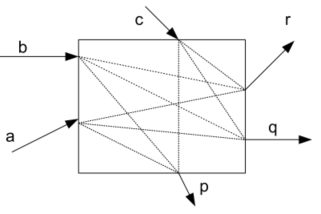
\includegraphics[width=0.35\textwidth]{Bilder/MixZone.PNG}
		\caption{Mix-Zone Model, Quelle: \protect\cite{Palanisamy2011}}
		\label{fig_Palanisamy2011}
\end{figure}

\cite{Palanisamy2011} definiert das eine Mix-Zone Z k-anonymisierend für eine Menge von Nutzern A ist wenn folgende Bedingungen erfüllt sind:
\begin{enumerate}
\item Die Menge A hat mindestens k Elemente, $ |A| \geq k $.
\item Alle Nutzer in A müssen die Mix-Zone Z betreten haben, bevor ein Nutzer aus A die Mix-Zone Z verlässt.
\item Jeder Nutzer der Menge A die Mix-Zone durch einen Eintrittspunkt betritt $ e_{i} \in E $ und diese durch einen Austrittspunkt $ o_{i} \in O $ verlässt und dabei eine zufällige Zeitspanne in der Zone verweilt.
\item Die Übergangswahrscheinlichkeit von jeden Eintrittspunkt zu jeden Austrittspunkt folgt einer Gleichverteilung.
\end{enumerate}
\subsection{Mix-Zones über Straßennetze (Lars Taubmann)} \label{sec:mixZonesStrasse}
\cite{Palanisamy2011} beschreibt, dass die vorher betrachtete Definition der Mix-Zone davon ausgeht, dass sich die bewegenden Nutzer frei in einem euklidischen Raum bewegen, ohne dass sie von räumlichen Beschränkungen betroffen sind. Im Normalfall in der Alltagswelt der mobilen Nutzer ist dies nicht so. So sind sie zum Beispiel durch Straßennetze und Fußgängerwege in ihrer freien Bewegung eingeschränkt. Die Mix-Zones für Straßennetze werden in der Regel einer Straßenkreuzung zugeordnet. Welche Straßenkreuzung als Standort einer Mix-Zone geeignet ist, hängt gewöhnlich von einer Reihe von Faktoren ab. Diese Faktoren beinhalten die Anzahl an Straßen, die an einer Kreuzung zusammen laufen, die Geschwindigkeit der mobilen Nutzer, und Pfadbeschränkungen für mobile Nutzer, die sich innerhalb einer Mix-Zone aufhalten. Ebenso beeinflussen die ausgewählten Kreuzungen, auf denen Mix-Zones errichtet werden sollen, auch die Anzahl der Eintritts- und Austrittspunkte der Mix-Zone, da diese die eingehenden und ausgehenden Straßensegmente abbilden müssen und somit die Anzahl an Eintritts- und Austrittspunkten begrenzen. Auch liegen die Nutzer unter Beschränkungen durch das Straßennetz innerhalb einer Mix-Zone: Sie müssen sich an Geschwindigkeitsbegrenzungen halten und auch ihre freie Bewegung auf Grund von Straßen- und Gehsteigsführung ist eingeschnitten. Daraus resultiert, dass Punkt (1), das zufällig Lange Aufhalten in einer Mix-Zone, und Punkt (2), die Gleichverteilung der Übergangswahrscheinlichkeiten von Eintritts- und Austrittspunkten, in der Definition der k-Anonymität einer Mix-Zone verletzt werden. In den folgenden Absätzen wird erläutert, wie sich diese beiden Verletzungen nach \cite{Chow2011} der k-Anonymität auf den Grad der Anonymität auswirken.

\begin{figure}[!h]
	\centering
	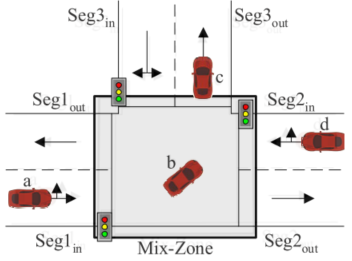
\includegraphics[width=0.4\textwidth]{Bilder/MixZoneNetwork.PNG}
	\caption{Mix-Zone eines Straßennetzwerks, Quelle: \protect\cite{Chow2011}}
	\label{fig_MixSrasse}
\end{figure}

1)	\textit{Mix-Zones ohne zufälliges Aufenthalten in ihr}: Sobald Nutzer eine unbestimmte Zeit in der Mix-Zone aufhalten, stellt eine zufällige Umordnung zwischen der Eintrittsreihenfolge und der Austrittsreihenfolge eine starke Unverknüpfbarkeit zwischen alten und neuen Pseudonymen sicher. Zum Beispiel, wenn alle Nutzer eine konstante Zeit in einer Mix-Zone verbringen, würde das System dem einfachen First-In-First-Out Prinzip entsprechen. Und somit kann dem ersten verlassenden Pseudonym das entsprechende erste eintretende Pseudonym zugeordnet werde und so weiter.

2)	\textit{Mix-Zones ohne gleichverteilte Übergangswahrscheinlichkeiten}: Sobald die Regel gelockert wird, dass die Übergangswahrscheinlichkeit zwischen Eintritts- und Austrittspunkt gleichverteilt sind wie in der theoretischen Mix-Zone, können einige Übergange zwischen Ein- und Austrittspunkten wahrscheinlicher werden als andere. Ein Angreifer könnte dieses Wissen nutzen, um  Verknüpfungen zwischen neuen und alten Pseudonymen zu folgern. Beispielhaft könnte ein Angreifer in einen solchen Szenario Übergänge, die weniger wahrscheinlich sind, aus seiner Abbildung der Pseudonyme entsprechend dieser Übergänge eliminieren und somit das Inferieren der Pseudonymverknüpfungen verbessern.

Aus diesen beiden Schwächen leitet \cite{Palanisamy2015} die drei Arten von Attacken auf Mix-Zones über Straßennetzwerken ab: (1) Timing Attacks, (2) Transaction Attacks und (3) Combined Timing and Transition Attacks.

1)	\textit{Timing Attack}: Bei einer Timing Attack beobachtet der Angreifer die Eintritts- $t_{in}(i)$ und die Austrittszeit $t_{out}(i)$ für jeden Nutzer der die Mix-Zone durchquert. Sobald der Angreifer erkennt das ein Nutzer i' die Mix-Zone verlässt, versucht er i' auf einen Nutzer aus dem Anonymitätsmenge A$_{i}$ ab zu bilden. Der Angreifer weißt der Wahrscheinlichkeit $p_{i'\rightarrow j}$ einen Wert zu, so dass dieser der Wahrscheinlichkeit i' auf j abzubilden entspricht, wobei $j \in A$. Die Abbildungswahrscheinlichkeiten werden berechnet durch Inferenz, basierend auf den Wahrscheinlichkeiten von den übriggebliebenen Nutzer, das diese zum Austrittszeitpunkt $t_{out}(i')$ die Mix-Zone verlassen. Nachdem die Abbildungswahrscheinlichkeiten berechnet worden sind, kann der Angreifer die Schiefe in der Abbildungswahrscheinlichkeitsverteilung nutzen, um Abbildungen mit geringer Wahrscheinlichkeit  unter Abwägung zu entfernen und so die Anzahl der Nutzer aus A, die in Betracht kommen, durch die Berücksichtigung von hoch wahrscheinlichen Abbildungen einzugrenzen.

2)	\textit{Transition Attack}: Bei einer Transition Attack schätzt der Angreifer die Übergangswahrscheinlichkeit für jede Abbiegemöglichkeit auf Grundlage vorheriger Beobachtungen. Beim Erkennen, dass ein Nutzer i' die Mix-Zone verlässt, weißt der Angreifer der Abbildungswahrscheinlichkeit $p_{i'\rightarrow j}$  für jedes $j \in A$ auf Grundlage der Bedingten Übergangswahrscheinlichkeiten T(iseg(i), oseg(i')) und T(iseg(j), oseg(i')).  T(iseg(j), oseg(i')) ist dabei die Notation der Bedingten Wahrscheinlichkeit eines Nutzers i' der durch Straßensegment iseg(j) die Mix-Zone betreten hat unter der Bedingung diese über das Straßensegment oseg(i') verlassen hat. Die Abbildungswahrscheinlichkeiten  $p_{i'\rightarrow i}$ und $p_{i'\rightarrow j}$ unter einer Transition Attack sind daher durch \\
$p_{i'\rightarrow i} = \dfrac{T(iseg(i), oseg(i'))}{T(iseg(i), oseg(i')) + T(iseg(j), oseg(i'))} $\\
und \\
$p_{i'\rightarrow j} = \dfrac{T(iseg(j), oseg(i'))}{T(iseg(i), oseg(i')) + T(iseg(j), oseg(i'))} $ \\ gegeben.

3)	\textit{Combined  Timing and Transition Attack}: Bei dieser Art von Angriff ist der Angreifer sowohl wissend über die Ein- und Austrittszeiten der Nutzer als auch den Übergangswahrscheinlichkeiten an Kreuzungen der gegebenen Mix-Zone des Straßennetzwerks. Der Angreifer kann  daher die Abbildungswahrscheinlichkeit $p_{i'\rightarrow j}$ für jedes $j \in A$ basierend auf den Wahrscheinlichkeiten des Nutzers j zum Zeitpunkt $t_{out}(i')$ die Mix-Zone verlässt und den bedingten Übergangswahrscheinlichkeiten $T(iseg(j), oseg(i'))$ schätzen. 

\begin{figure}[!h]
	\centering
	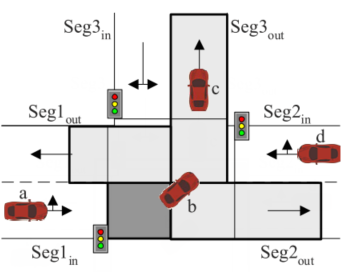
\includegraphics[width=0.4\textwidth]{Bilder/nonrectangularMix.PNG}
	\caption{Non-Rectangular Mix-Zone, Quelle: \protect\cite{Chow2011}}
	\label{fig_MixSrasseNon}
\end{figure}

Da eine einfache rechteckige Mix-Zone um eine Straßenkreuzung diesen Attacken nicht ausreichend stand hält, haben \cite{Palanisamy2015} und \cite{Palanisamy2011} die Time Window Bounded Non-Rectangular Mix-Zones entworfen. Dieser Typ von Mix-Zone besteht aus mehreren rechteckigen Teilstücken.  Diese beginnen von der Mitte der Kreuzung und liegen nur auf den ausgehenden Straßensegmenten der Kreuzung (siehe Abbildung \ref{fig_MixSrasseNon}). Dieser Ansatz wird im Folgenden als Non-Rectangular Ansatz bezeichnet. Dieser Ansatz schützt besser vor Timing Attacks, die auf der Heterogenität der Geschwindigkeitsverteilung auf den Straßensegmenten basieren. Es wird angenommen, das sie Anonymitätsmenge für jeden Nutzer i alle Nutzer beinhaltet, die die Mix-Zone in einem Zeitfenster mit dem Intervall $| t_{in}(i)-\tau_{1}|$ bis $|t_{in}(i)+\tau_{2}|$ betreten haben. $t_{in}(i)$ ist der Eintrittszeitpunkt des Nutzers i und t$_{a1}$ und t$_{a2}$ werden als so kleine Werte gewählt, dass das Zeitfenster sicherstellt, dass die Anonymitätsmenge von i nur Nutzer ähnlich naher Ankunftszeit beinhaltet. Die Länge der Mix-Zone auf den ausgehenden Straßensegmenten  wird basierend auf der Geschwindigkeit des Straßensegments, der Größe des Zeitfensters und dem benötigten Anonymitätsgrad bestimmt.     
\subsection{False Locations (Tina Kämmerer)} \label{sec:falseLocations}
Die Verwendung von Dummy Trajectories hat jedoch auch einige Nachteile. Zum einen entsteht ein Overhead bei jeder Anfrage, da sowohl beim Nutzer und bei eventueller Middleware, als auch bei den LBS, viele zusätzliche Ressourcen für die Erstellung und Bearbeitung der Dummies benötigt werden. Im Gegensatz zu Dummy Positions ist die Generierung von realistischen Dummy Trajectories, die nicht von realen Trajectories unterschieden werden können, relativ anspruchsvoll \cite{Beresford2003}.


\subsubsection{Pseudonyme und Middleware} \label{subsubsection:pseudomiddle}
Ein anderer Ansatz, um die Privatsphäre von LBS-Nutzern zu gewährleisten, wird durch die Kombination von Dummy Locations und einem Application Server realisiert \cite{Sahu2012}. Hierbei gibt es einige Ähnlichkeiten mit den Mix Zones \cite{Beresford2003}, bei denen Nutzer über Middleware anonymisiert werden, indem sie für die Aufenthaltsdauer in einem definierten räumlichen Bereich ein Pseudonym annehmen und auf Positionsupdates verzichten. Somit kann der Nutzer nicht von anderen Personen in der Mix Zone differenziert werden und es ist ebenso keine Verbindung zwischen dem Eintritt und Austritt eines Nutzers aus der Mix Zone herstellbar. Es ergibt sich jedoch der Nachteil, dass durch die nicht akkurate Positionsangabe auch die Qualität der LBS abnimmt. 
Bei dem vorgestellten Ansatz wird ebenfalls Middleware eingesetzt, die dem Nutzer Pseudonyme zuweist, die nach einem bestimmten Zeitraum geändert werden. Anders als bei den Mix Zones übermittelt der Nutzer jedoch weiterhin Positionsupdates an die LBS, um einen bestmöglichen Service zu erhalten. Jedoch ist dadurch der alleinige Einsatz von mehreren aufeinander folgenden Pseudonymen für die Privatsphäre nicht ausreichend, da durch Inferenz eine Verknüpfung zwischen diesen hergestellt werden könnte. Deshalb generiert der Nutzer eine Reihe von Dummy Locations, welche zusätzlich zu der realen Position über die Middleware an die LBS übermittelt werden. Damit steht den LBS eine genaue Position zur Verfügung, um Ergebnisse für die Anfrage zu generieren, gleichzeitig bleibt die Identität des Nutzers jedoch unbekannt. Aus den Ergebnissen der Anfrage kann der Nutzer nun die für ihn relevanten Informationen selektieren.
Abhängig von der Anzahl der generierten Dummies K und den mit der Zeit wechselnden Pseudonyme N für jeden Nutzer in einer Zeit T entstehen somit K$^{N}$ verschiedene Pfade für jeden Benutzer. Die Variable K kann somit Abhängig von dem gewünschten Anonymitätsgrad und der zur Verfügung stehenden Processing Power gewählt werden.

\begin{table*}[!ht]
\centering
\renewcommand{\arraystretch}{1.6}
\caption{Vergleich verschiedener Anonymisierungsansätze}
\label{table:vergleich1}
\begin{threeparttable}
    \begin{tabular}{{l|cccccc}}
    	~ & LBS I / LBS II   & Processing Power & Overhead 	& Relocatable 	& Involved Parties & Trusted Services \\ \hline
    	Mix-Zone           & Nein / Ja & ? & Niedrig & Nein & n User & Ja \\
    	Vehicular Mix-Zone & Nein / Ja & ? & Niedrig & Nein & n User & Ja \\
    	Spatial Cloaking: Distortion & Ja / Ja & Mittel & Hoch & Ja & n User & Ja \\
    	Spatial Cloaking: Prediction & Ja / Ja & Hoch   & Hoch & Ja & n User & Ja \\
	    False Locations I (\ref{para:simple})     				& Ja / Ja          & Mittel   		  & Mittel      & Ja           	& 1 User\tnote{a}    & Nein			  \\
		False Locations II (\ref{para:modul})     				& Ja / Ja          & Mittel   		  & Niedrig      & Ja           	& 1 User    		   & Nein\tnote{b}			  \\
    	False Locations III (\ref{para:middle})    				& Nein / Ja        & Hoch     		  & Hoch        & Ja            & 1 User             & Middleware	      \\
    \end{tabular}
    \begin{tablenotes}
    	\item[a] Daten von anderen Usern verbessern Ergebnis
    	\item[b] Benötigt zusätzliches Modul bei LBS-Server
    \end{tablenotes}
    \end{threeparttable}
\end{table*}


\section{Analysis} \label{sec:analysis}
\begin{table*}[!ht]
\renewcommand{\arraystretch}{1.3}
\caption{Vergleich verschiedener Anonymisierungsansätze}
\label{table:vergleich1}
\centering
    \begin{tabular}{{l|llllll}}
    	~                    								& LBS I / LBS II   & Processing Power & Overhead 	& Relocatable 	& Involved Parties & Trusted Services \\ \hline
    	Spatial Cloaking     								& ~                & ~                & ~        	& ~           	& ~                & ~                \\
    	Space Transformation 								& ~                & ~                & ~        	& ~           	& ~                & ~                \\
	    False Locations \ref{subsubsection:realdummy}     	& Ja / Ja          & Middle   		  & Middle      & Ja           	& User*            & Nein			  \\
    	False Locations \ref{subsubsection:pseudomiddle}    & Nein / Ja        & High     		  & High        & Ja            & User             & Middleware	      \\
    \end{tabular}
\end{table*}
\section{Conclusion} \label{sec:conclusion}
Conclusion
\bibliographystyle{IEEEtran}
\bibliography{Literature}
\end{document}


% An example of a floating figure using the graphicx package.
% Note that \label must occur AFTER (or within) \caption.
% For figures, \caption should occur after the \includegraphics.
% Note that IEEEtran v1.7 and later has special internal code that
% is designed to preserve the operation of \label within \caption
% even when the captionsoff option is in effect. However, because
% of issues like this, it may be the safest practice to put all your
% \label just after \caption rather than within \caption{}.
%
% Reminder: the "draftcls" or "draftclsnofoot", not "draft", class
% option should be used if it is desired that the figures are to be
% displayed while in draft mode.
%
%\begin{figure}[!t]
%\centering
%\includegraphics[width=2.5in]{myfigure}
% where an .eps filename suffix will be assumed under latex, 
% and a .pdf suffix will be assumed for pdflatex; or what has been declared
% via \DeclareGraphicsExtensions.
%\caption{Simulation Results}
%\label{fig_sim}
%\end{figure}

% Note that IEEE typically puts floats only at the top, even when this
% results in a large percentage of a column being occupied by floats.


% An example of a double column floating figure using two subfigures.
% (The subfig.sty package must be loaded for this to work.)
% The subfigure \label commands are set within each subfloat command, the
% \label for the overall figure must come after \caption.
% \hfil must be used as a separator to get equal spacing.
% The subfigure.sty package works much the same way, except \subfigure is
% used instead of \subfloat.
%
%\begin{figure*}[!t]
%\centerline{\subfloat[Case I]\includegraphics[width=2.5in]{subfigcase1}%
%\label{fig_first_case}}
%\hfil
%\subfloat[Case II]{\includegraphics[width=2.5in]{subfigcase2}%
%\label{fig_second_case}}}
%\caption{Simulation results}
%\label{fig_sim}
%\end{figure*}
%
% Note that often IEEE papers with subfigures do not employ subfigure
% captions (using the optional argument to \subfloat), but instead will
% reference/describe all of them (a), (b), etc., within the main caption.


% An example of a floating table. Note that, for IEEE style tables, the 
% \caption command should come BEFORE the table. Table text will default to
% \footnotesize as IEEE normally uses this smaller font for tables.
% The \label must come after \caption as always.
%
%\begin{table}[!t]
%% increase table row spacing, adjust to taste
%\renewcommand{\arraystretch}{1.3}
% if using array.sty, it might be a good idea to tweak the value of
% \extrarowheight as needed to properly center the text within the cells
%\caption{An Example of a Table}
%\label{table_example}
%\centering
%% Some packages, such as MDW tools, offer better commands for making tables
%% than the plain LaTeX2e tabular which is used here.
%\begin{tabular}{|c||c|}
%\hline
%One & Two\\
%\hline
%Three & Four\\
%\hline
%\end{tabular}
%\end{table}


% Note that IEEE does not put floats in the very first column - or typically
% anywhere on the first page for that matter. Also, in-text middle ("here")
% positioning is not used. Most IEEE journals/conferences use top floats
% exclusively. Note that, LaTeX2e, unlike IEEE journals/conferences, places
% footnotes above bottom floats. This can be corrected via the \fnbelowfloat
% command of the stfloats package.






% conference papers do not normally have an appendix




% trigger a \newpage just before the given reference
% number - used to balance the columns on the last page
% adjust value as needed - may need to be readjusted if
% the document is modified later
%\IEEEtriggeratref{8}
% The "triggered" command can be changed if desired:
%\IEEEtriggercmd{\enlargethispage{-5in}}

% references section

% can use a bibliography generated by BibTeX as a .bbl file
% BibTeX documentation can be easily obtained at:
% http://www.ctan.org/tex-archive/biblio/bibtex/contrib/doc/
% The IEEEtran BibTeX style support page is at:
% http://www.michaelshell.org/tex/ieeetran/bibtex/
%\bibliographystyle{IEEEtran}
% argument is your BibTeX string definitions and bibliography database(s)
%\bibliography{IEEEabrv,../bib/paper}
%
% <OR> manually copy in the resultant .bbl file
% set second argument of \begin to the number of references
% (used to reserve space for the reference number labels box)



